\documentclass{article}
\usepackage{a4wide}
\usepackage[english]{babel}
\usepackage[latin1]{inputenc}
\selectlanguage{english}
\usepackage{amsmath,url,graphics,verbatim}
\DeclareGraphicsRule{*}{mps}{*}{}

\begin{document}

\title{An example of automaton generated\\with the MetaPost package \url{automata.mp}}
\author{Gabriele Puppis\\
        \url{gabriele.puppis@gmail.com}}

\maketitle

This \LaTeX\ document shows how to include a picture generated with MetaPost.
By default, the extension of a file generated with MetaPost is a number
(e.g., \url{.0}), so you should use the package \url{graphics} and the command 
\verb \DeclareGraphicsRule{*}{mps}{*}{}  to make \LaTeX\ recognize these 
extensions as files in PS format. 

The file \url{example.mp} contains the MetaPost source code that was used to generate 
the automaton in Figure \ref{fig:example}. This file should be compiled with MetaPost 
(e.g., run ``\verb mp  \verb -tex=latex  \verb example.mp '' from the shell command 
line). Such an example uses the package \url{automata.mp} to easily draw the states 
and the transitions of the automaton (you can find some documentation inside the files 
\url{example.mp} and \url{automata.mp}).

\begin{figure}[!!h]
\centering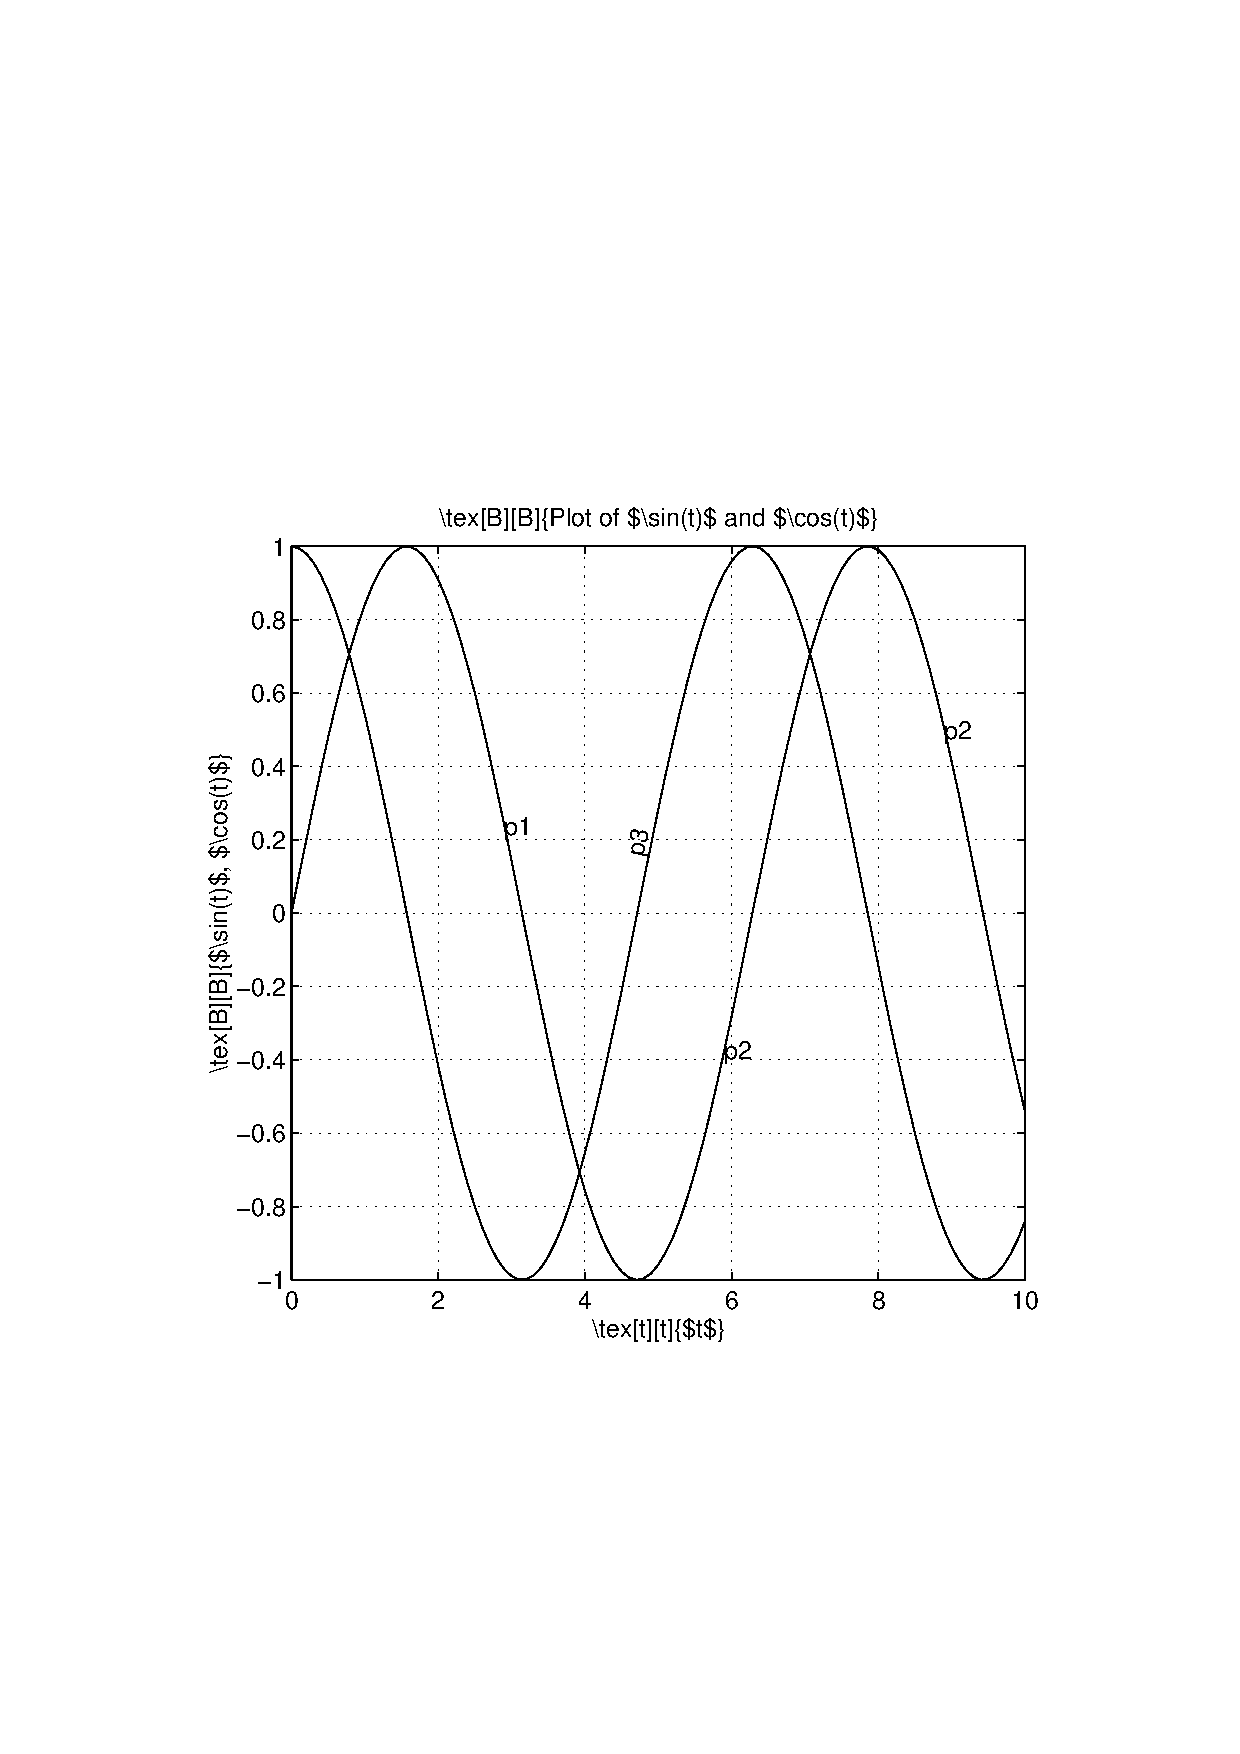
\includegraphics{example.0}
\caption{An example of automaton}\label{fig:example}
\end{figure}

\end{document}